\DiaryEntry{Nonlinear Dynamics and Chaos, 1}{2015-11-01}{Maths}

Based on the book ``Nonlinear Dynamics and Chaos'' from Strogatz.

\subsection{One-dimensional Flows}

Consider a (one-dimensional) function $x(t)$ and we are given its derivative (with respect to t) in terms of a function $f(x)$. Note that $f(x)$ does \emph{not} depend on the time parameter $t$:

\[
\frac{dx(t)}{dt} = f(x)
\]

There may only be a numerical solution to this differential equation; however, the expression provides insights into the solution(s). Upon drawing the relation between $x$ and $\frac{dx(t)}{dt}$, we can find intervals of $x$, where the derivative is (i) positive and therefore $x(t)$ will increase, (ii) is negative and therefore $x(t)$ will decrease, and (iii) is zero and therefore $x(t)$ will stay constant (if $\frac{dx(t)}{dt} = 0$ for $x=x^\star$, then $x(t)=x^\star$). The latter points / regions are called fixed points.

\subsubsection{Stability of Fixed Points}

Assume $x^\star$ is a fixed point. If $\frac{dx(t)}{dt} < 0$ for $x > x^\star$, then $x(t)$ will increase. Similarly, if $\frac{dx(t)}{dt} > 0$ for $x < x^\star$, then $x(t)$ will decrease. In short, if $x$ deviates from the fixed point, the derivative will ``pull'' it back towards the fixed point $x^\star$. Such a fixed point is called a stable fixed point. The condition on the behavior of $\frac{dx(t)}{dt}$ around the fixed point is equivalent to a negative slope of $\frac{dx(t)}{dt}$.

Conversely, if the derivative ``pushes'' away from the fixed point ($\frac{dx(t)}{dt} > 0$ for $x > x^\star$ and $\frac{dx(t)}{dt} < 0$ for $x < x^\star$), the fixed point is called an unstable one. This is equivalent to a positive slope of $\frac{dx(t)}{dt}$.

This can be seen as a one-dimensional vector field on the x-axis; the
direction and length of the vectors are given by $f(x)$. The Figure below shows an example of a system with one stable fixed point $x_1$ (the slope is negative) and an unstable fixed point $x_2$ (the slope
is positive).

\begin{figure}[H]
\centering
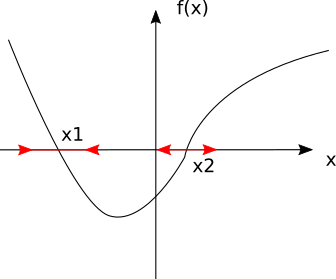
\includegraphics{images/strogatz_1_1.png}
\caption{Page1}
\end{figure}

In a one-dimensional system, the solutions $x(t)$ either approach a fixed point or diverge to $\pm \infty$. No oscillations are possible.


\subsubsection{Example}

We have

\[
\frac{df}{dx} = \sin(x)
\]

Fixed points are at location $x^\star = k \pi$ with stable fixed points at odd $k$ (here the slope is negative) and unstable fixed points at even $k$ (the slope being positive).

\subsection{Two-dimensional Flows}

Here we have two functions $x=x(t), y=y(t)$ with system equations as follows:


\begin{align*}
\frac{dx}{dt} & = f(x,y) \\
\frac{dy}{dt} & = g(x,y)
\end{align*}


In order to visualize what is going on, we use phase plane which is a
two- dimensional vector field with components $(f(x,y), g(x,y))^T$. The trajectories of the phase plane describe possible solutions: An actual solution starts at some initial value $(x\_0, y\_0)$ and then moves along the trajectory. The norm of the vector $(f(x,y), g(x,y))^T$ can be interpreted as the speed with which the vector field is traversed.

With this interpretation, a norm of zero implies no movement along the trajectory; in other words, the solution has arrived at a fixed point. The norm of a vector becomes only zero when all components vanish. Therefore, a fixed point is a point $(x^\star,y^\star)$ for which $f(x^\star, y^\star) = g(x^\star,y^\star) = 0$.

Depending on the starting point, the trajectory may end up in a fixed
point, diverge, or oscillate in the phase plane.

There is a result that such systems of differential equations always
have a unique solution (which may depend on initial values). Therefore, trajectories will never intersect. If there would be an intersection, then two solutions would start from the same point (the intersection) which would violate the uniqueness constraint.

An immediate consequence is, that if there is a closed trajectory
$\mathcal{C}$ in the phase plane, it separates the trajectories into an ``inside'' and ``outside''. The ``inside'' trajectories cannot cross $\mathcal{C}$ and get ``outside''; vice versa for the ``outside trajectories'' which cannot get ``inside''.


\subsubsection{Stability of Fixed Points}

To analyze fixed points, the Jacobian matrix of the system is used. The Jacobian is defined as

\[ J(x,y) = \left( \begin{array}{cc}
\frac{\partial f(x,y)}{\partial x} & \frac{\partial f(x,y)}{\partial y}  \\
\frac{\partial g(x,y)}{\partial x} & \frac{\partial g(x,y)}{\partial y}
\end{array} \right) \]

Based on the values of the Jacobian eigenvalues, the following
distinction is made:

\begin{itemize}
\item
  If both eigenvalues have positive real part, the fixed point is an
  unstable point and repels trajectories.
\item
  If both eigenvalues have negative real part, the fixed point is a
  stable point and attracts trajectories.
\item
  If one eigenvalue is positive and the other negative, the fixed point   is a saddle point.
\item
  If both eigenvalues are imaginary, one or both eigenvalues are zero, the fixed point is a center / higher order point.
\end{itemize}

If there are several stable fixed points in a system, the $x-y$-space can be separated into several basins: All initial points $(x_0, y_0)$ which eventually ($t \rightarrow \infty$) end up in the same fixed point belong into the same basin.


\subsubsection{Example}

Consider the following system

\begin{align*}
\frac{dx}{dt} & = x(3-x-2y) \\
\frac{dy}{dt} & = y(2-x-y)
\end{align*}

Setting the LHS to zero in both equations, we get 4 fixed points:
$(0,0), (0,2), (3,0), (1,1$.

The Jacobian has the following form

\bee
J(x,y) = \left(
\begin{bmatrix}{cc}
3-2x-2y & -2x  \\
-y & 2-x-2y  
\end{bmatrix}
\right)
\eee

In the following we will calculate the Jacobi matrix for the 4 fixed
points and analyze the Jacobian's eigenvalues.

\begin{itemize}
\item
  Fixed point $(0,0)$: The Jacobian becomes \[J(x,y) = \left(
  \begin{array}{cc} 3 & 0  \\ 0 & 2 \end{array} \right) \] with
  eigenvalues 3 and 2. They are positive, therefore the fixed point is a repelling one.
\item
  Fixed point $(0,2)$: The Jacobian becomes \[J(x,y) = \left(
  \begin{array}{cc} -1 & 0  \\ -2 & -2 \end{array} \right) \] with two negative eigenvalues (-1 and -2). Therefore the fixed point is an attracting one.
\item
  Fixed point $(3,0)$: The Jacobian becomes \[J(x,y) = \left(
  \begin{array}{cc} -3 & -6  \\ 0 & -1 \end{array} \right) \] with two   negative eigenvalues (-1 and -3). Therefore the fixed point is an attracting one.
\item
  Fixed point $(1,1)$: The Jacobian becomes \[J(x,y) = \left(
  \begin{array}{cc} -1 & -2  \\ -1 & -1 \end{array} \right) \] with one   negative and one positive eigenvalue ($-1 \pm \sqrt{2}$). Therefore the fixed point is a saddle point.
\end{itemize}

The Figure below shows the (numerically obtained) phase portrait which supports the calculations together with the 4 fixed points.

\begin{figure}[H]
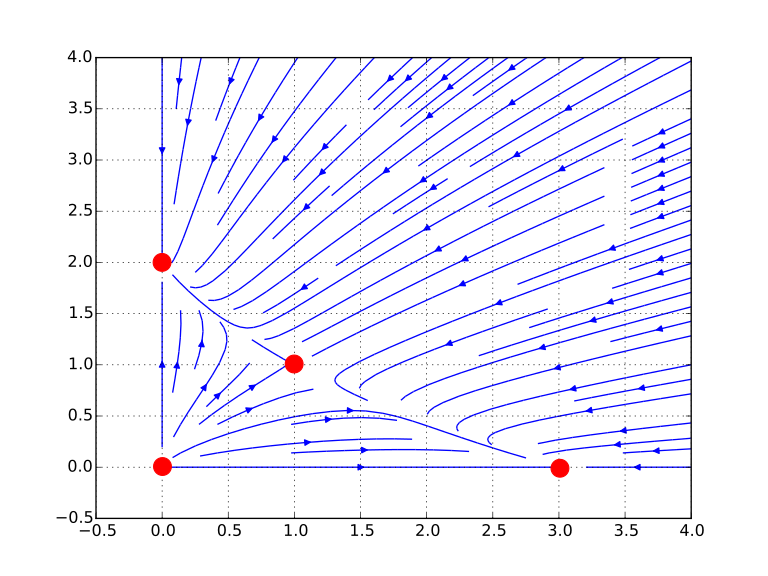
\includegraphics[scale=0.7]{images/strogatz_1_2.png}
\end{figure}

The Figure below shows the example trajectory starting at $(3,3)$ being ``swallowed'' by the fixed point $(0,2)$.

\begin{figure}[H]
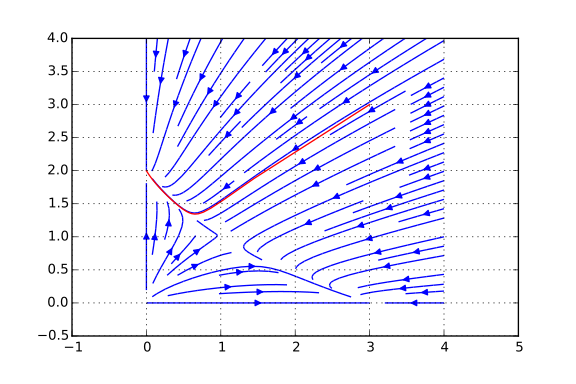
\includegraphics[scale=0.7]{images/strogatz_1_3.png}
\end{figure}

The corresponding plots of $x(t)$ and $y(t)$ as functions of
$t$ have the following form

\begin{figure}[H]
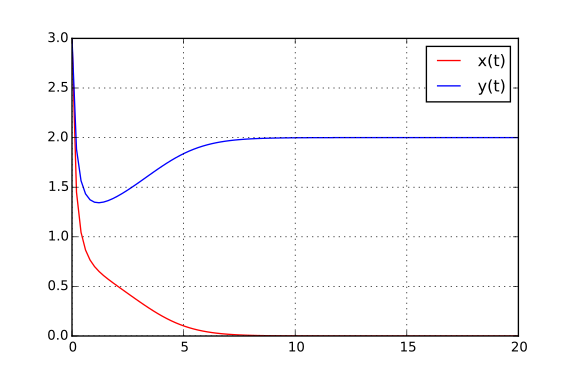
\includegraphics[scale=0.7]{images/strogatz_1_4.png}
\end{figure}

The function $y(t)$ makes a ``dip'' to $\approx 1.4$ before it converges to $2$. $x(t)$ converges to zero with ``two velocities''; before the ``dip'' the rate of decrease is larger than afterwards.
